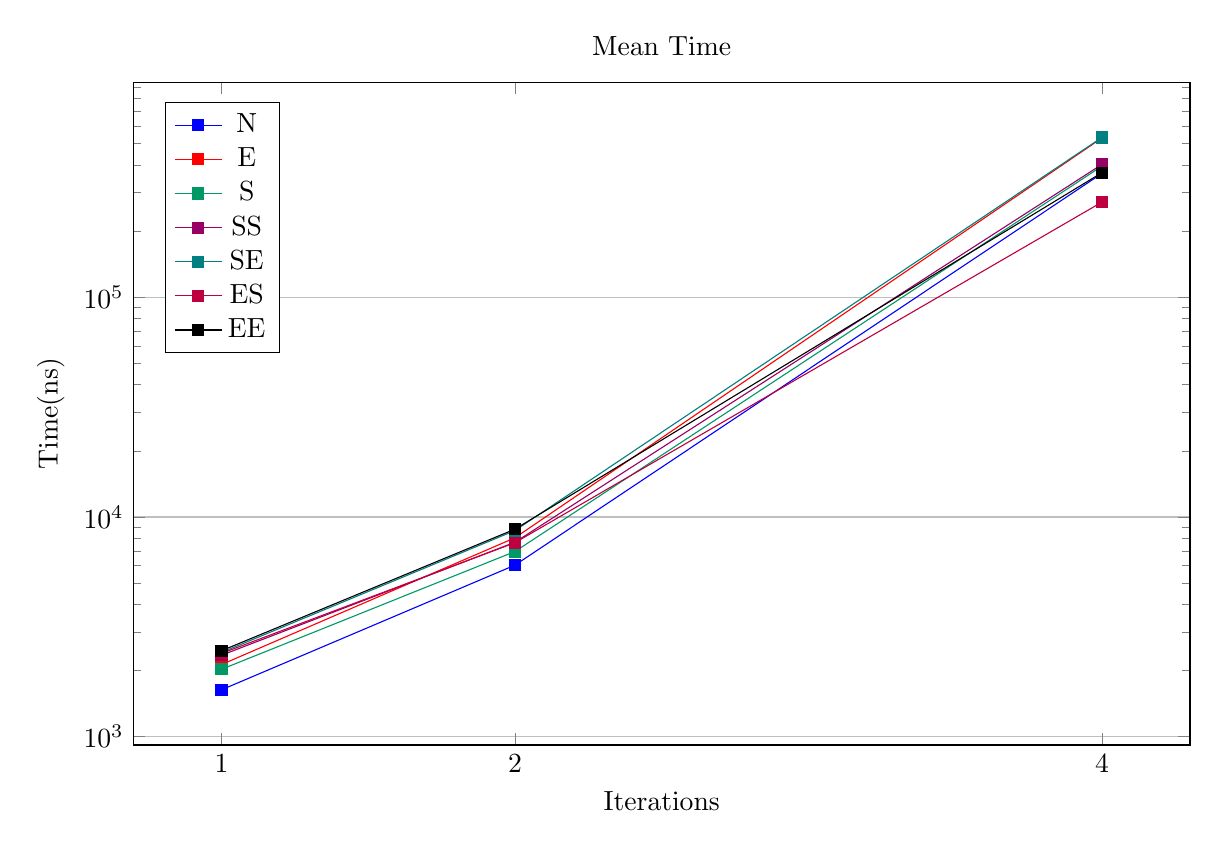
\begin{tikzpicture}
    \begin{semilogyaxis}[
            title={Mean Time},
            width=15cm,
            height=10cm,
            ymin=0,
            legend pos=north west,
            xlabel={Iterations},
            ylabel={Time(ns)},
            xtick={1,2,4},
            ymajorgrids=true,
        ]

        \addplot[color=blue, mark=square*] coordinates {(1,1634.9)(2,6036.6)(4,365861.8)};
        \addlegendentry{N}
        \addplot[color=red, mark=square*] coordinates {(1,2130.0)(2,8039.4)(4,530259.4)};
        \addlegendentry{E}
        \addplot[color=green!60!blue, mark=square*] coordinates {(1,2027.1)(2,6962.4)(4,394797.3)};
        \addlegendentry{S}
        \addplot[color=red!60!blue, mark=square*] coordinates {(1,2348.2)(2,7674.8)(4,402027)};
        \addlegendentry{SS}
        \addplot[color=teal, mark=square*] coordinates {(1,2417.8)(2,8672.8)(4,533352.9)};
        \addlegendentry{SE}
        \addplot[color=purple, mark=square*] coordinates {(1,2394.1)(2,7637.9)(4,270858.2)};
        \addlegendentry{ES}
        \addplot[color=black, mark=square*] coordinates {(1,2461.5)(2,8800.2)(4,368669.7)};
        \addlegendentry{EE}
    \end{semilogyaxis}
\end{tikzpicture}